\chapter{RNA Tak Penyandi dan Pengaturan Pascatranskripsi}\label{ch:b3:rna-regulation}

Pada tahun 1990 dua ahli biologi tumbuhan mencoba membuat petunia lebih ungu
dengan memberinya salinan tambahan gen enzim pigmennya. Hampir separuh
tumbuhan transgenik itu keluar berwarna putih, atau ungu dengan sektor putih:
gen tambahan tersebut telah mematikan salinan milik tumbuhan itu sendiri
sekaligus mematikan dirinya. Delapan tahun kemudian, dua ahli genetika cacing
yang menyuntikkan RNA ke dalam \emph{Caenorhabditis elegans} mendapati bahwa
RNA beruntai ganda yang cocok dengan sebuah gen otot membungkam gen itu, pada
cacing yang disuntik maupun pada keturunannya, jauh lebih ampuh daripada
masing-masing untainya sendiri. Kedua teka-teki itu berjawaban satu: sel
memiliki permesinan yang memakai RNA pendek untuk menemukan dan membungkam
RNA yang urutannya cocok. Permesinan itu, dan dunia pengaturan yang lebih
luas yang menimpa sebuah RNA duta sesudah ditranskripsi --- bagaimana ia
disambung, ke mana ia dikirim, berapa lama ia hidup, apakah ia
ditranslasi --- adalah pokok bab ini. Jilid Tahun 1 memperlakukan gen sebagai
satuan yang menyala atau padam pada promotornya; di sini transkripnya sendiri
yang menjadi sasaran kendali.

\section{Sensus RNA sebuah sel}

\begin{definition}[RNA tak penyandi]\label{def:b3:rna-regulation:ncrna}
\index{RNA tak penyandi}\index{mikroRNA}\index{siRNA}%
\index{piRNA}\index{RNA tak penyandi panjang}\index{RNA nukleus kecil}
Sebuah \emph{RNA tak penyandi} (ncRNA) adalah transkrip yang bekerja sebagai
RNA, bukan sebagai cetakan bagi protein. Di luar RNA ribosom dan RNA pemindah
dalam translasi serta \emph{RNA nukleus kecil} (snRNA) milik spliseosom,
sebuah sel eukariot memuat: \emph{mikroRNA} (miRNA), \numrange{21}{23}
nukleotida, yang dipotong dari jepit rambut di dalam transkrip sel itu sendiri
dan memandu penekanan RNA duta yang sebagian komplementer; \emph{RNA
pengganggu kecil} (siRNA), sepanjang itu juga, yang dipotong dari RNA beruntai
ganda yang panjang dan memandu pemotongan sasaran yang cocok sempurna;
\emph{RNA yang berinteraksi dengan Piwi} (piRNA), \numrange{26}{31}
nukleotida, yang aktif di dalam garis nutfah melawan transposon; RNA nukleolus
kecil yang memandu modifikasi rRNA; dan \emph{RNA tak penyandi panjang}
(lncRNA), transkrip yang lebih panjang daripada \qty{200}{nt} tanpa kerangka
baca terbuka yang berarti, yang di antaranya \emph{\omterm{def:b3:chromatin-epigenetics:x-inactivation}{Xist}} pada
\cref{ch:b3:chromatin-epigenetics} paling dipahami. Ekson penyandi protein
menempati sekitar \qty{1.5}{\%} genom manusia; sebagian besar sisanya
ditranskripsi pada suatu saat di dalam suatu sel, tetapi berapa banyak
transkripsi itu yang berfungsi masih menjadi pertanyaan terbuka.
\end{definition}

\begin{remark}[Kelimpahan bukan fungsi]\label{rem:b3:rna-regulation:function}
Sebuah transkrip dapat terdeteksi karena polimerasenya bocor, bukan karena
RNA-nya mengerjakan sesuatu; sebagian besar lncRNA hadir kurang dari satu
salinan tiap sel, tidak lestari, dan dapat ditiadakan tanpa akibat. Uji
fungsinya bersifat genetik: adanya fenotipe ketika RNA-nya, dan bukan sekadar
DNA-nya, dibuang. \emph{\omterm{def:b3:chromatin-epigenetics:x-inactivation}{Xist}}, miRNA, dan \omterm{def:b3:rna-regulation:ncrna}{piRNA} melewatinya dengan
meyakinkan; dari puluhan ribu lncRNA yang teranotasi, sejauh ini baru
beberapa ratus yang melewatinya.
\end{remark}

\section{Interferensi RNA dan mikroRNA}

\begin{definition}[Interferensi RNA]\label{def:b3:rna-regulation:rnai}
\index{interferensi RNA}\index{Dicer}\index{Argonaute}\index{RISC}
\emph{Interferensi RNA} (RNAi) adalah pembungkaman sebuah gen yang khas
urutan oleh RNA kecil yang berasal dari RNA beruntai ganda. Enzim
\emph{Dicer}, sebuah RNase III, memotong RNA beruntai ganda yang panjang
menjadi duplek sepanjang \numrange{21}{23} nukleotida dengan tonjolan 3$'$
sepanjang dua nukleotida; salah satu untai tiap duplek, yaitu pemandunya,
dimuatkan ke dalam protein \emph{Argonaute} sehingga membentuk
\emph{kompleks pembungkam terimbas RNA} (RISC). Pemandunya berpasangan dengan
RNA sasaran yang komplementer, dan domain endonuklease Argonaute memotong
sasarannya berhadapan dengan nukleotida 10 dan 11 pemandunya; RNA yang
terpotong lalu diuraikan dan RISC-nya dilepaskan untuk mencari sasaran lain.
Pada tumbuhan, cacing, dan fungi sebuah RNA polimerase bergantung-RNA
menyalin sasarannya menjadi RNA beruntai ganda yang baru, sehingga isyaratnya
diperkuat dan menyebar; mamalia tidak memiliki langkah ini.
\end{definition}

\begin{proof}[Bukti eksperimental]
Napoli, Lemieux, dan Jorgensen (1990) memasukkan satu gen kalkon sintase
tambahan ke dalam petunia untuk memekatkan warna bunganya; \qty{42}{\%}
transformannya berwarna putih atau belang, dengan transgen maupun gen
endogennya sama-sama dibungkam --- ``kosupresi''. Guo dan Kemphues (1995)
mendapati bahwa RNA antisens terhadap sebuah gen \emph{C.~elegans}
membungkamnya, tetapi kendali sensnya pun berbuat sama. Fire, Mello, dan
rekan (1998) menuntaskan paradoks itu: sediaan untai tunggal mereka tercemar
untai ganda, dan RNA beruntai ganda \emph{unc-22} yang telah dimurnikan lalu
disuntikkan ke dalam seekor cacing memberi fenotipe \emph{unc-22} yang
berkedut pada kepekatan beberapa molekul tiap sel, sedangkan RNA sens atau
antisens murni hampir tidak memberi apa-apa; pembungkamannya menyeberang ke
jaringan yang jauh dari tempat suntikan dan ke keturunannya. Hamilton dan
Baulcombe (1999) mendeteksi RNA \qty{25}{nt} di dalam tumbuhan yang
terbungkam, dan Zamore serta rekan (2000) menunjukkan pada ekstrak lalat
bahwa RNA beruntai ganda itu terpotong menjadi RNA tersebut dan bahwa
sasarannya terpotong pada selang \qty{21}{nt}.
\end{proof}

\begin{omfigure}
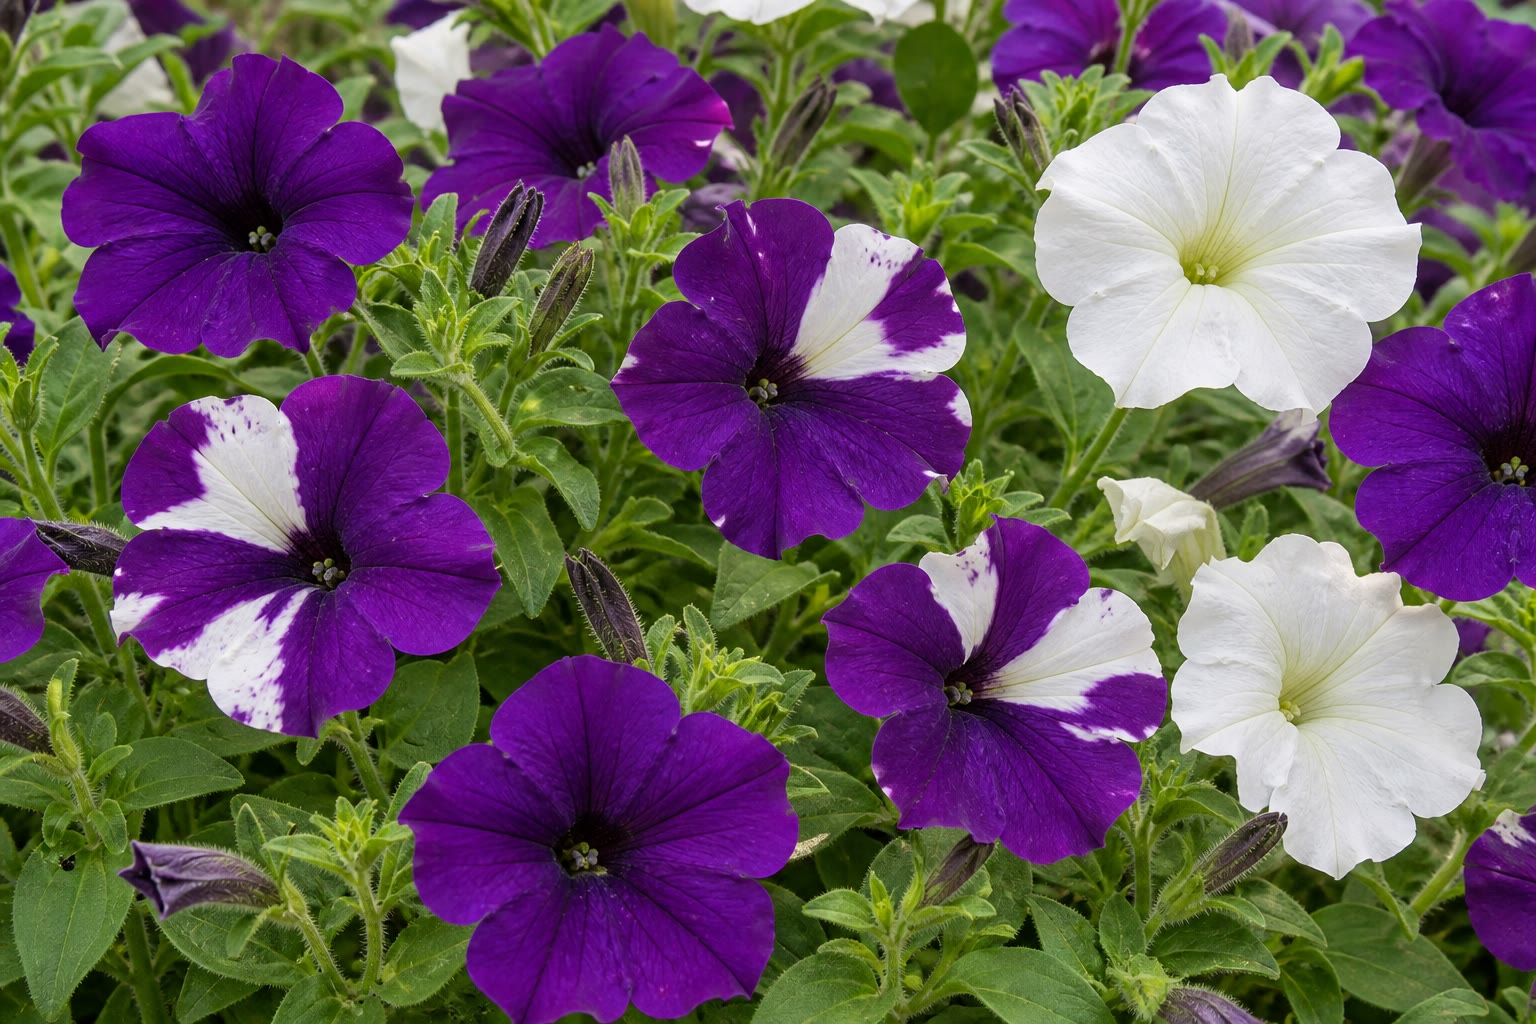
\includegraphics[width=0.46\linewidth]{images/book5/ai/b5-02-petunia-cosuppression.jpg}\hspace{0.04\linewidth}
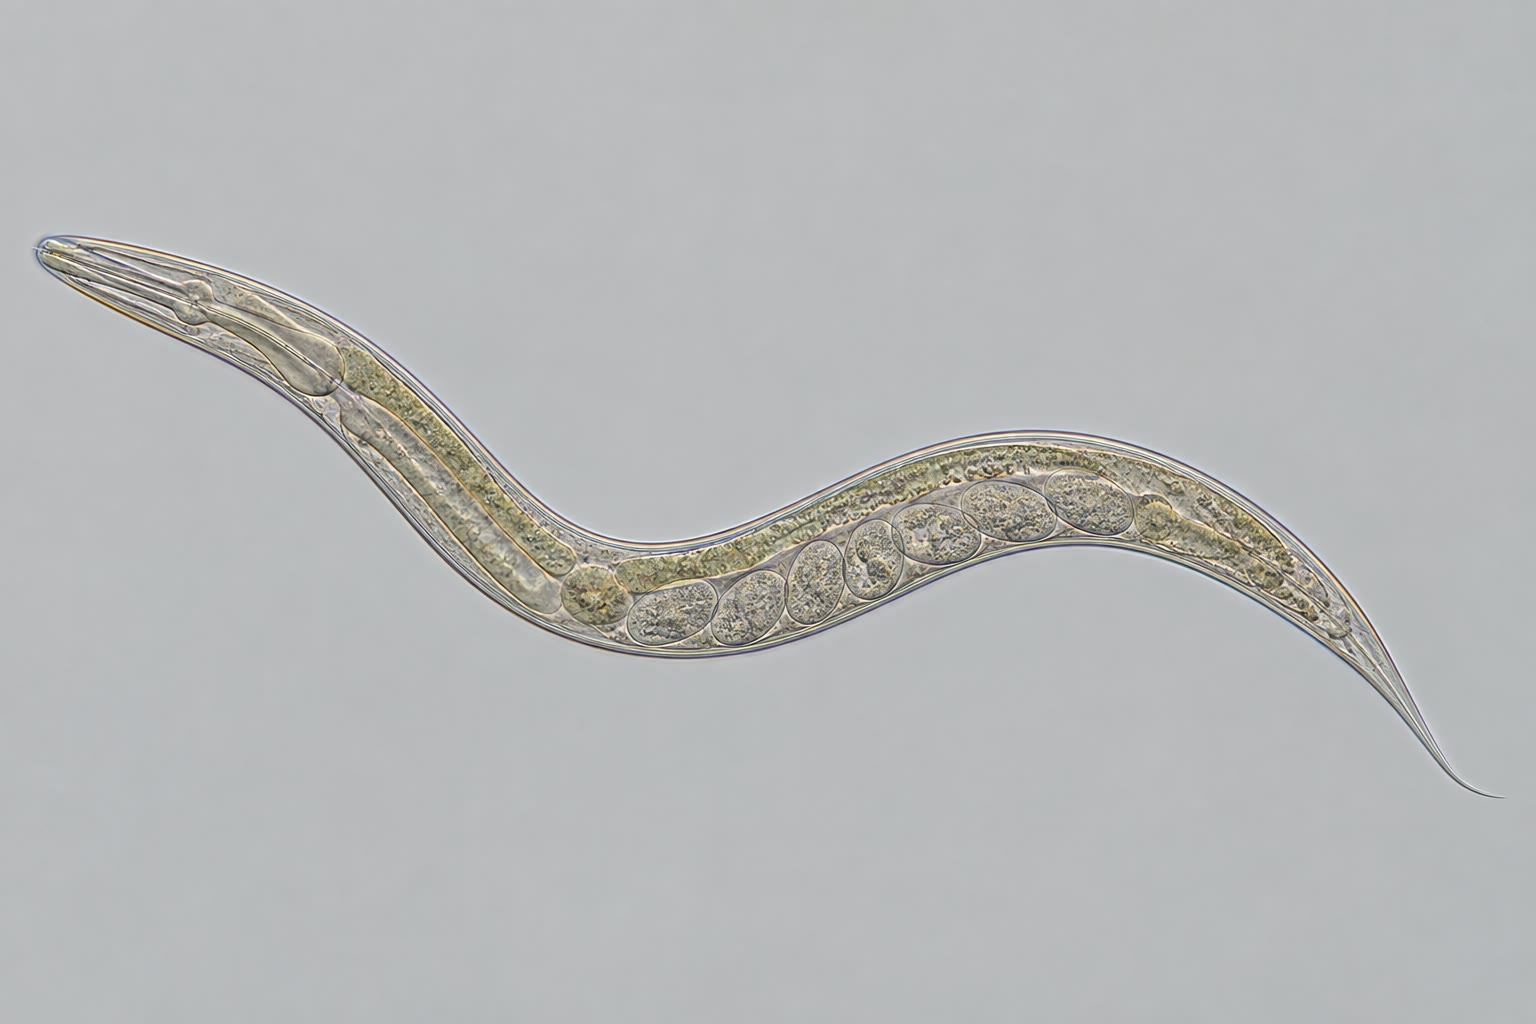
\includegraphics[width=0.46\linewidth]{images/book5/ai/b5-02-c-elegans.jpg}

{\small Kiri: petunia yang membawa satu gen pigmen tambahan, dengan sektor
putih hasil kosupresi. Kanan: nematoda \emph{Caenorhabditis elegans},
sepanjang kira-kira satu milimeter dan bening, yang di dalamnya RNA beruntai
ganda suntikan membungkam gen yang cocok pada seluruh tubuh hewan itu dan
pada keturunannya.}
\end{omfigure}

\begin{definition}[MikroRNA]\label{def:b3:rna-regulation:mirna}
\index{mikroRNA!biogenesis}\index{Drosha}\index{urutan benih}
Sebuah \emph{\omterm{def:b3:rna-regulation:ncrna}{mikroRNA}} disandikan di dalam genom --- pada gennya sendiri atau
di dalam intron sebuah gen penyandi protein --- lalu ditranskripsi oleh RNA
polimerase II sebagai transkrip primer yang panjang (pri-miRNA) yang memuat
jepit rambut sepanjang kira-kira \qty{70}{nt}. Di dalam nukleus, RNase III
bernama \emph{Drosha}, bersama pasangannya DGCR8, memotong jepit rambut itu
keluar (pre-miRNA); eksportin-5 membawanya ke sitoplasma, tempat \omterm{def:b3:rna-regulation:rnai}{Dicer}
membuang lengkungnya sehingga tersisa duplek \qty{22}{nt}. Satu untainya
dimuatkan ke dalam \omterm{def:b3:rna-regulation:rnai}{Argonaute}. MiRNA yang matang mengenali sasarannya terutama
lewat \emph{benih}-nya, yakni nukleotida 2 sampai 8, yang berpasangan dengan
tapak yang lazimnya berada di daerah tak tertranslasi 3$'$ sebuah RNA duta;
sisa miRNA-nya berpasangan tak sempurna, sehingga sasarannya tidak dipotong
melainkan ditekan: \omterm{def:b3:rna-regulation:rnai}{RISC-nya} merekrut protein yang memendekkan ekor poli(A),
membuang tudungnya, dan menghambat translasi, dan RNA dutanya diuraikan lebih
cepat. Karena sebuah benih hanya tujuh nukleotida, satu miRNA memiliki ratusan
sasaran, dan lebih dari separuh gen penyandi protein manusia mengusung tapak
lestari bagi sedikitnya satu dari beberapa ratus miRNA manusia yang telah
terkenali dengan yakin.
\end{definition}

\begin{proof}[Bukti eksperimental]
\emph{lin-4}, sebuah gen yang dibutuhkan cacing untuk beranjak dari tahap
larva pertamanya ke tahap kedua, ditemukan Lee, Feinbaum, dan Ambros (1993)
menyandikan bukan sebuah protein melainkan RNA \qty{22}{nt}, yang komplementer
dengan tujuh tapak di daerah tak tertranslasi 3$'$ RNA duta \emph{lin-14},
yakni gen yang telah diketahui ditekannya. Ketika larvanya memasuki tahap
kedua, protein LIN-14 lenyap sedangkan mRNA-nya tetap ada: penekanannya
bersifat pascatranskripsi. Reinhart dan rekan (2000) menemukan RNA kedua
semacam itu, \emph{let-7}, yang mengendalikan peralihan larva berikutnya;
Pasquinelli (2000) menemukan \emph{let-7} pada lalat dan manusia, dengan
urutan yang sama, dan itulah yang mengubah keanehan cacing menjadi mekanisme
umum.
\end{proof}

\begin{omfigure}
\begin{tikzpicture}[every node/.style={font=\scriptsize}, >=stealth]
  % nucleus box
  \draw[rounded corners=8pt, thick, gray!60, fill=gray!6] (-0.4,-1.1) rectangle (5.2,2.7);
  \node[gray, anchor=south west] at (-0.3,-1.05) {nukleus};
  % gene and pri-miRNA
  \draw[very thick, omDef] (0,2.0) -- (2.4,2.0); \node[above] at (1.2,2.05) {gen miRNA, Pol II};
  \draw[->, thick] (1.2,1.85) -- (1.2,1.35);
  % hairpin
  \draw[thick, omThm!70!black] (0.2,1.0) -- (0.9,1.0) .. controls (1.0,1.0) and (1.05,0.9) .. (1.1,0.5) .. controls (1.15,0.1) and (1.25,0.1) .. (1.3,0.5) .. controls (1.35,0.9) and (1.4,1.0) .. (1.5,1.0) -- (2.2,1.0);
  \draw[thick, omThm!70!black] (1.1,0.5) -- (1.3,0.5);
  \node[below] at (1.2,0.0) {jepit rambut pri-miRNA};
  % Drosha
  \draw[thick, fill=omExo!35] (2.9,0.7) ellipse (0.55 and 0.28); \node at (2.9,0.7) {Drosha};
  \draw[->, thick] (2.3,0.85) -- (2.4,0.75);
  \draw[->, thick] (3.5,0.7) -- (4.2,0.7) node[midway, above] {potong};
  % pre-miRNA
  \draw[thick, omThm!70!black] (4.3,0.9) .. controls (4.5,0.9) and (4.55,0.4) .. (4.6,0.1) .. controls (4.65,-0.2) and (4.75,-0.2) .. (4.8,0.1) .. controls (4.85,0.4) and (4.9,0.9) .. (5.1,0.9);
  \node[below, align=center] at (4.7,-0.25) {pre-miRNA\\\qty{70}{nt}};
  % export
  \draw[->, thick] (5.35,0.4) -- (6.3,0.4) node[midway, above, xshift=0.2cm] {eksportin-5};
  % cytoplasm
  \node[gray, anchor=north west] at (5.5,2.65) {sitoplasma};
  \draw[thick, fill=omExo!35] (6.9,0.4) ellipse (0.5 and 0.28); \node at (6.9,0.4) {Dicer};
  \draw[->, thick] (7.45,0.4) -- (8.1,0.4);
  \draw[thick, omThm!70!black] (8.2,0.55) -- (9.6,0.55); \draw[thick, omThm!70!black] (8.35,0.25) -- (9.75,0.25);
  \node[below, align=center] at (8.95,0.15) {duplek \qty{22}{nt}};
  \draw[->, thick] (8.95,-0.4) -- (8.95,-0.9) node[midway, right] {satu untai dimuatkan};
  % RISC on mRNA
  \draw[thick, fill=omProp!35] (8.95,-1.45) ellipse (0.85 and 0.35); \node at (8.95,-1.45) {Argonaute};
  \draw[thick, omThm!70!black] (8.3,-1.85) -- (9.6,-1.85);
  \draw[very thick, omDef] (5.6,-2.15) -- (11.4,-2.15);
  \node[below] at (6.4,-2.2) {mRNA: daerah penyandi}; \node[below] at (10.3,-2.2) {UTR 3$'$, tapak sasaran};
  \draw[omDef, thick] (11.4,-2.15) -- (11.8,-2.15) node[right] {AAAA};
  \draw[->, thick, omThm] (9.9,-1.5) -- (10.9,-1.5) node[right, align=left] {deadenilasi,\\peluruhan, translasi\\berkurang};
  \node[below, align=center] at (8.95,-2.7) {benih (nt 2--8) berpasangan\\dengan tapaknya};
\end{tikzpicture}

{\small Biogenesis sebuah \omterm{def:b3:rna-regulation:ncrna}{mikroRNA}. Jepit rambutnya dipotong keluar dari
transkrip primernya oleh \omterm{def:b3:rna-regulation:mirna}{Drosha} di dalam nukleus, diekspor, dirapikan oleh
\omterm{def:b3:rna-regulation:rnai}{Dicer} menjadi duplek \qty{22}{nt}, dan satu untainya dimuatkan ke dalam
\omterm{def:b3:rna-regulation:rnai}{Argonaute}. Benihnya berpasangan dengan sebuah tapak di daerah tak
tertranslasi 3$'$ sebuah RNA duta, lalu RNA duta itu dideadenilasi, diuraikan,
dan lebih jarang ditranslasi.}
\end{omfigure}

\begin{theorem}[Apa yang dilakukan mikroRNA pada kadar dan kecepatan sebuah RNA duta]\label{thm:b3:rna-regulation:mirna-kinetics}
\index{waktu paruh mRNA}\index{waktu tanggap}
Sebuah RNA duta disintesis dengan laju tetap $k$ dan diuraikan dengan laju
orde satu $\gamma$; sebuah \omterm{def:b3:rna-regulation:ncrna}{mikroRNA} yang hadir pada kadar $R$ menambahkan
suku peluruhan $\gamma' R\, m$. Maka kadar mRNA $m(t)$ memenuhi
\[
\frac{\mathrm{d}m}{\mathrm{d}t} = k - (\gamma + \gamma' R)\, m,
\qquad
m^{*} = \frac{k}{\gamma + \gamma' R},
\qquad
m(t) = m^{*} + (m_{0} - m^{*})\,e^{-(\gamma + \gamma' R)t}.
\]
\omterm{def:b3:rna-regulation:ncrna}{MikroRNA} itu menurunkan keadaan tunaknya dengan faktor $1 + \gamma' R/
\gamma$ dan memendekkan tetapan waktu setiap perubahan $m$ dari
$1/\gamma$ menjadi $1/(\gamma + \gamma' R)$ dengan faktor yang sama. Sebuah
gen yang diatur \omterm{def:b3:rna-regulation:ncrna}{mikroRNA} karena itu sekaligus lebih tenang dan lebih cepat:
ia mencapai keadaan tunak yang baru lebih cepat sesudah promotornya berubah,
dan riak dalam transkripsinya teredam.
\end{theorem}
\begin{proof}
Persamaannya linear dengan koefisien tetap; titik tetapnya adalah $m^{*}$,
tempat ruas kanannya lenyap, dan dengan menulis $u = m - m^{*}$ diperoleh
$\mathrm{d}u/\mathrm{d}t = -(\gamma + \gamma' R)\,u$, sehingga muncul
eksponensialnya. Waktu paruh pendekatannya adalah $\ln 2/(\gamma + \gamma'
R)$, dan $\gamma = \ln 2 / t_{1/2}$ dengan $t_{1/2}$ waktu paruh alami RNA
duta itu.
\end{proof}

\begin{example}[Penekanan empat kali lipat]\label{ex:b3:rna-regulation:fourfold}
Sebuah RNA duta yang waktu paruh alaminya \qty{30}{min} ($\gamma =
\qty{0.023}{min^{-1}}$), yang ditranskripsi pada $k = 2$ molekul tiap menit,
berada pada $m^{*} = 2/0.023 \approx 87$ salinan tiap sel dan memerlukan
\qty{30}{min} untuk beranjak separuh jalan menuju kadar baru sesudah
promotornya berubah. Sebuah \omterm{def:b3:rna-regulation:ncrna}{mikroRNA} yang melipattigakan laju peluruhannya
($\gamma' R = 3\gamma$) membawanya ke $22$ salinan dan memangkas waktu
paruhnya menjadi \qty{7.5}{min}. Angka yang sama, dibaca terbalik,
memperlihatkan mengapa penidakaktifan miRNA sering berfenotipe ringan:
perubahan empat kali lipat pada RNA duta yang dirinya sendiri teredam di
hilir dapat meninggalkan organismenya hampir normal, dan pengaruhnya baru
tampak di bawah cekaman atau pada penataan waktunya.
\end{example}

\begin{omfigure}
\begin{tikzpicture}
\begin{axis}[
  width=0.7\linewidth, height=5.6cm,
  axis x line=bottom, axis y line=left,
  xmin=0, xmax=120, ymin=0, ymax=100,
  xlabel={waktu sesudah promotor menyala (min)}, ylabel={mRNA tiap sel},
  xlabel style={font=\small, at={(axis description cs:0.5,-0.12)}, anchor=north},
  ylabel style={font=\small},
  tick label style={font=\small}, xtick={0,30,60,90,120}, ytick={0,22,50,87},
  clip=false,
]
\addplot[very thick, omDef, domain=0:120, samples=80] {87*(1-exp(-0.0231*x))};
\addplot[very thick, omThm, domain=0:120, samples=80] {21.7*(1-exp(-0.0924*x))};
\addplot[dashed, gray, domain=0:120, samples=2] {87};
\addplot[dashed, gray, domain=0:120, samples=2] {21.7};
\node[font=\scriptsize, omDef, anchor=south west] at (axis cs:5,90) {tanpa mikroRNA: $m^{*} = 87$, waktu paruh \qty{30}{min}};
\node[font=\scriptsize, omThm, anchor=south west] at (axis cs:40,24) {dengan mikroRNA, $\gamma' R = 3\gamma$: $m^{*} = 22$, waktu paruh \qty{7.5}{min}};
\end{axis}
\end{tikzpicture}

{\small Naiknya sebuah RNA duta sesudah promotornya dinyalakan, dengan angka
\cref{ex:b3:rna-regulation:fourfold}. \omterm{def:b3:rna-regulation:ncrna}{MikroRNA} itu menurunkan
dataran tingginya empat kali lipat dan mencapainya empat kali lebih cepat.}
\end{omfigure}

\begin{method}[Meredam sebuah gen dengan RNAi]\label{met:b3:rna-regulation:knockdown}
\index{peredaman gen}\index{shRNA}
Untuk membungkam sebuah gen tanpa menyentuh DNA-nya: (1) pilihlah urutan
\qty{21}{nt} yang khas bagi RNA dutanya, sambil menghindari kecocokan benih
dengan gen lain; (2) antarkanlah urutan itu sebagai duplek \omterm{def:b3:rna-regulation:ncrna}{siRNA} sintetik
(sementara, beberapa hari) atau sebagai RNA jepit rambut pendek (shRNA) yang
diekspresikan dari sebuah vektor, yang terus-menerus diolah \omterm{def:b3:rna-regulation:rnai}{Dicer}; pada
cacing, berilah hewannya makan bakteri yang mengekspresikan RNA beruntai
ganda itu; (3) ukurlah RNA dutanya dengan PCR kuantitatif dan proteinnya
dengan imunoblot, sambil mengharapkan kehilangan \qtyrange{70}{95}{\%}, bukan
ketiadaan lengkap seperti pada penidakaktifan gen; (4) kendalikanlah pengaruh
di luar sasaran dengan \omterm{def:b3:rna-regulation:ncrna}{siRNA} kedua yang tak bertindihan dan dengan penyelamatan
oleh versi gen yang kebal RNAi. Peredaman adalah kehilangan fungsi yang
sebagian dan berbalik; terapi gen yang kini disetujui atas asas ini
mengantarkan \omterm{def:b3:rna-regulation:ncrna}{siRNA} terhadap RNA duta hati (transtiretin, PCSK9) yang
digandengkan pada gula yang diserap hepatosit.
\end{method}

\section{RNA kecil yang menjaga genom}

\begin{definition}[piRNA dan pembungkaman transposon]\label{def:b3:rna-regulation:pirna}
\index{piRNA!ping-pong}\index{pembungkaman transposon}\index{disgenesis hibrid}
\emph{\omterm{def:b3:rna-regulation:ncrna}{piRNA}} adalah RNA sepanjang \numrange{26}{31} nukleotida, dibuat tanpa
\omterm{def:b3:rna-regulation:rnai}{Dicer} dari transkrip beruntai tunggal yang panjang milik \emph{gugus \omterm{def:b3:rna-regulation:ncrna}{piRNA}}
genomik --- kuburan salinan transposon yang cacat --- lalu dimuatkan ke dalam
anak suku PIWI protein \omterm{def:b3:rna-regulation:rnai}{Argonaute} di dalam garis nutfah. Sebuah \omterm{def:b3:rna-regulation:ncrna}{piRNA} yang
antisens terhadap sebuah transposon memandu pemotongan transkrip transposon
itu; fragmen yang terpotong menjadi \omterm{def:b3:rna-regulation:ncrna}{piRNA} sens yang baru, yang pada gilirannya
memotong transkrip gugusnya untuk membuat lebih banyak \omterm{def:b3:rna-regulation:ncrna}{piRNA} antisens ---
daur \emph{ping-pong}, sebuah penguatan yang menyasar transposon mana pun yang
sedang aktif. Protein PIWI di dalam nukleus juga mengarahkan metilasi H3K9 dan
\omterm{def:b3:chromatin-epigenetics:methylation}{metilasi DNA} ke salinan genomik transposon itu, sehingga RNA-nya terhubung
dengan tanda \omterm{def:b3:chromatin-epigenetics:nucleosome}{kromatin} \cref{ch:b3:chromatin-epigenetics}. Seekor induk
menitipkan \omterm{def:b3:rna-regulation:ncrna}{piRNA-nya} di dalam telur; betina yang garis keturunannya belum
pernah berjumpa dengan sebuah transposon tidak memiliki \omterm{def:b3:rna-regulation:ncrna}{piRNA} terhadapnya,
dan keturunannya dari jantan yang membawa transposon itu mandul ---
\emph{disgenesis hibrid}, yang mula-mula terlihat pada persilangan
\emph{Drosophila} antara galur laboratorium dan galur liar.
\end{definition}

\begin{proposition}[Pembungkaman kromatin terarah RNA]\label{prop:b3:rna-regulation:rddm}
\index{metilasi DNA terarah RNA}
Pada tumbuhan, sebuah jalur khusus --- RNA polimerase IV mentranskripsi
sebuah lokus, RNA polimerase bergantung-RNA membuatnya beruntai ganda, sebuah
\omterm{def:b3:rna-regulation:rnai}{Dicer} memotong \omterm{def:b3:rna-regulation:ncrna}{siRNA} \qty{24}{nt}, \omterm{def:b3:rna-regulation:rnai}{Argonaute}~4 membawanya kembali ke
transkrip nasen polimerase V pada lokus yang sama lalu merekrut
metiltransferase DRM2 --- memetilasi DNA transposon dan urutan berulang;
jalur itulah mekanisme paramutasi. Pada khamir belah, \omterm{def:b3:rna-regulation:ncrna}{siRNA} dari urutan
berulang sentromer merekrut metiltransferase H3K9 dan membangun \omterm{def:b3:chromatin-epigenetics:nucleosome}{heterokromatin}
yang dibutuhkan sentromernya. Pada kedua kasus itu sebuah RNA menemukan
tempatnya di dalam genom lewat kekomplementeran, lalu sebuah tanda \omterm{def:b3:chromatin-epigenetics:nucleosome}{kromatin}
dituliskan di situ: khas urutan, memperkuat diri, dan diwariskan sepanjang
pembelahan.
\end{proposition}

\section{Riwayat hidup sebuah RNA duta}

\begin{definition}[Penyambungan yang diatur]\label{def:b3:rna-regulation:splicing}
\index{penyambungan alternatif!pengaturan}\index{protein SR}%
\index{hnRNP}\index{pelewatan ekson}
Penyambungan alternatif menghasilkan RNA duta yang berlainan dari satu gen
lewat \emph{pelewatan ekson}, pilihan antara ekson yang saling meniadakan,
penahanan sebuah intron, atau pemakaian tapak sambung 5$'$ maupun 3$'$
alternatif. Semuanya diatur oleh protein pengikat RNA yang mengikat unsur
urutan di dalam ekson dan intron dekat sebuah tapak sambung: \emph{protein
SR} yang terikat pada penguat eksonik merekrut spliseosom dan memacu
penyertaan eksonnya, protein \emph{hnRNP} yang terikat pada pembungkam
menghalanginya, dan hasilnya pada sebuah sel ditentukan oleh jumlah nisbi
kedua macam protein itu. Lebih dari \qty{90}{\%} gen manusia bereksonrangkap
disambung secara alternatif; gen \emph{Dscam} \emph{Drosophila}, dengan
empat blok ekson yang saling meniadakan (12, 48, 33, dan 2 pilihan), dapat
menghasilkan \num{38016} protein berbeda, dan tiap neuron mengekspresikan
perangkat yang berlainan sehingga cabangnya saling mengenali dan menghindar.
\end{definition}

\begin{proof}[Bukti eksperimental]
Jenis kelamin lalat buah diputuskan oleh sebuah riam penyambungan. Pada
betina gen \emph{Sex-lethal} (\emph{Sxl}) membuat protein yang berfungsi; SXL
adalah protein pengikat RNA yang menghalangi sebuah tapak sambung pada
transkripnya sendiri (sehingga ekson berkodon henti terlewat dan proteinnya
terus dibuat) dan pada transkrip \emph{transformer}, sehingga memaksa sambungan
betina; TRA, bersama TRA-2, lalu mengikat penguat eksonik pada transkrip
\emph{doublesex} dan mengarahkan bentuk betina faktor transkripsi DSX. Pada
jantan, tanpa SXL, setiap transkrip itu mengambil sambungan bakunya,
\emph{transformer} memuat kodon henti, dan DSX keluar dalam bentuk jantan.
Setiap ciri lalat yang dimorfik secara seksual mengikuti DSX mana yang
dibuat; betina yang \emph{tra}-nya dimutasikan berkembang sebagai jantan.
\end{proof}

\begin{definition}[Kemantapan dan penempatan mRNA]\label{def:b3:rna-regulation:stability}
\index{elemen kaya AU}\index{penempatan mRNA}%
\index{elemen tanggap besi}
\emph{Waktu paruh} sebuah RNA duta terentang dari beberapa menit sampai
beberapa hari dan ditentukan oleh unsur di daerah tak tertranslasi 3$'$-nya.
\emph{Elemen kaya AU} (ulangan AUUUA) di dalam RNA duta sitokina, faktor
pertumbuhan, dan protoonkogen diikat oleh protein yang merekrut deadenilase
dan memberi waktu paruh \qtyrange{10}{30}{min}, sehingga letupan transkripsi
menghasilkan letupan protein dan tidak lebih; mutasi yang membuangnya
menimbulkan ekspresi berlebih dan, bagi sebagian protoonkogen, kanker.
\emph{Elemen penempatan}, yang kerap berstruktur, diikat oleh adaptor yang
menghubungkan RNA dutanya dengan sebuah motor: RNA duta \emph{bicoid} dan
\emph{oskar} dibawa ke kedua kutub telur lalat oleh dinein dan kinesin pada
mikrotubulus, RNA duta aktin $\beta$ ke tepi depan sebuah fibroblas, dan RNA
duta protein sinaps ke dalam dendrit, tempat semuanya ditranslasi sesuai
permintaan. \emph{Elemen tanggap besi} (IRE), sebuah tangkai--lengkung yang
diikat protein pengatur besi IRP1 dan IRP2 ketika besi langka, mengerjakan dua
tugas berlawanan dari dua kedudukan: di daerah tak tertranslasi 5$'$ RNA duta
feritin, IRP yang terikat menghalangi ribosom; di daerah tak tertranslasi 3$'$
RNA duta reseptor transferin, IRP yang terikat melindungi transkripnya dari
sebuah nuklease.
\end{definition}

\begin{example}[Besi, yang dibaca satu jepit rambut]\label{ex:b3:rna-regulation:iron}
Ketika besi rendah, IRP mengikat kedua RNA duta itu: feritin, protein
simpanannya, tidak ditranslasi, dan reseptor transferin, yang mengimpor besi,
menjadi mantap dan melimpah --- selnya menyimpan lebih sedikit dan mengimpor
lebih banyak. Ketika besi tinggi, besi mengubah IRP1 menjadi akonitase (IRP1
memperoleh gugus besi--belerang dan kehilangan kegemarannya pada RNA) dan
memicu penguraian IRP2: feritin ditranslasi, RNA duta reseptornya meluruh
dalam hitungan menit, dan selnya menyimpan lebih banyak serta mengimpor lebih
sedikit. Tidak diperlukan perubahan transkripsi apa pun. Mutasi titik pada IRE
feritin yang mencegah pengikatan IRP menimbulkan sintesis feritin yang terus
berlangsung serta sindrom hiperferitinemia--katarak yang menurun.
\end{example}

\begin{omfigure}
\begin{tikzpicture}[every node/.style={font=\scriptsize}, >=stealth]
  \foreach \yy/\state in {2.2/besi rendah, -0.9/besi tinggi} {
    \node[left, font=\small\bfseries] at (-0.2,\yy+0.35) {\state};
    % ferritin mRNA
    \draw[very thick, omDef] (0.3,\yy+0.6) -- (4.6,\yy+0.6); \node[below] at (3.3,\yy+0.4) {mRNA feritin};
    \draw[thick, omThm!70!black] (0.9,\yy+0.6) .. controls (0.9,\yy+1.15) and (1.3,\yy+1.15) .. (1.3,\yy+0.6); \node[below] at (1.1,\yy+0.55) {IRE};
    \draw[fill=omDef!20, thick] (2.2,\yy+0.42) rectangle (4.4,\yy+0.78);
    % TfR mRNA
    \draw[very thick, omDef] (6.2,\yy+0.6) -- (10.6,\yy+0.6); \node[below, font=\tiny] at (7.1,\yy+0.4) {mRNA reseptor transferin};
    \draw[fill=omDef!20, thick] (6.4,\yy+0.42) rectangle (8.6,\yy+0.78);
    \foreach \x in {9.0,9.5,10.0} \draw[thick, omThm!70!black] (\x,\yy+0.6) .. controls (\x,\yy+1.1) and (\x+0.35,\yy+1.1) .. (\x+0.35,\yy+0.6);
    \node[below, font=\tiny] at (9.9,\yy+0.55) {IRE (UTR 3$'$)};
  }
  % low iron: IRP bound
  \draw[thick, fill=omProp!40] (1.1,3.35) ellipse (0.4 and 0.24); \node at (1.1,3.35) {IRP};
  \node[right, omThm] at (1.55,3.35) {ribosom terhalang: tanpa feritin};
  \foreach \x in {9.18,9.68,10.18} { \draw[thick, fill=omProp!40] (\x,3.35) ellipse (0.28 and 0.2); }
  \node[above, omMeth!70!black] at (9.7,3.75) {terlindung dari nuklease: reseptor mantap dan melimpah};
  \node[below, omMeth!70!black] at (1.1,1.75) {menyimpan lebih sedikit};
  \node[below, omMeth!70!black] at (7.4,1.75) {mengimpor lebih banyak};
  % high iron: IRP off
  \node[right, omMeth!70!black] at (1.55,0.25) {ditranslasi: feritin dibuat};
  \node[right, omThm, align=left] at (10.7,-0.3) {nuklease:\\mRNA meluruh};
  \node[below, omThm] at (1.1,-1.35) {menyimpan lebih banyak};
  \node[below, omThm] at (7.4,-1.35) {mengimpor lebih sedikit};
\end{tikzpicture}

{\small \omterm{def:b3:rna-regulation:stability}{Elemen tanggap besi}. Ketika besi rendah, protein pengatur besi
mengikat jepit rambut IRE: pada ujung 5$'$ RNA duta feritin protein itu
menghalangi translasi, pada ujung 3$'$ RNA duta reseptor transferin ia
menghalangi sebuah nuklease. Ketika besi tinggi protein itu melepaskan
keduanya: feritin dibuat, RNA duta reseptornya meluruh.}
\end{omfigure}

\begin{proposition}[Kendali translasi]\label{prop:b3:rna-regulation:translation}
\index{kendali translasi}\index{eIF2}\index{ribosakelar}\index{kerangka baca terbuka di hulu}
Langkah inisiasi adalah titik \omterm{prop:b3:rna-regulation:translation}{kendali translasi} yang lazim. Fosforilasi
faktor inisiasi \emph{eIF2} oleh kinase yang mengindera kelaparan asam amino,
protein yang salah melipat, RNA beruntai ganda virus, atau kekurangan hem
mematikan inisiasi umum dalam hitungan menit, sambil menyisakan beberapa RNA
duta yang berciri khusus --- terutama RNA duta ber\emph{\omterm{prop:b3:rna-regulation:translation}{kerangka baca terbuka
di hulu}}, yakni kerangka baca pendek di daerah tak tertranslasi 5$'$ yang
lazimnya memerangkap ribosom dan yang, di bawah cekaman, dilewati sehingga
faktor tanggap cekaman (GCN4 pada khamir, ATF4 pada mamalia) dibuat justru
ketika segala yang lain tidak. Faktor pengikat tudung eIF4E ditahan tak aktif
oleh protein pengikat 4E sampai kinase pengisyarat pertumbuhan mTOR
memfosforilasinya: sebuah sel mentranslasi dengan laju penuh hanya ketika
hara dan faktor pertumbuhan mengizinkannya. Pada bakteri, \emph{ribosakelar}
mengerjakannya tanpa protein apa pun: daerah 5$'$ yang berstruktur mengikat
sebuah metabolit (tiamina pirofosfat, S-adenosil metionina, sebuah purina)
dan, begitu terikat, melipat ulang sehingga mengubur tapak pengikat ribosom
atau membentuk terminator transkripsi, sehingga operon biosintesisnya padam
ketika hasilnya melimpah.
\end{proposition}

\begin{omfigure}
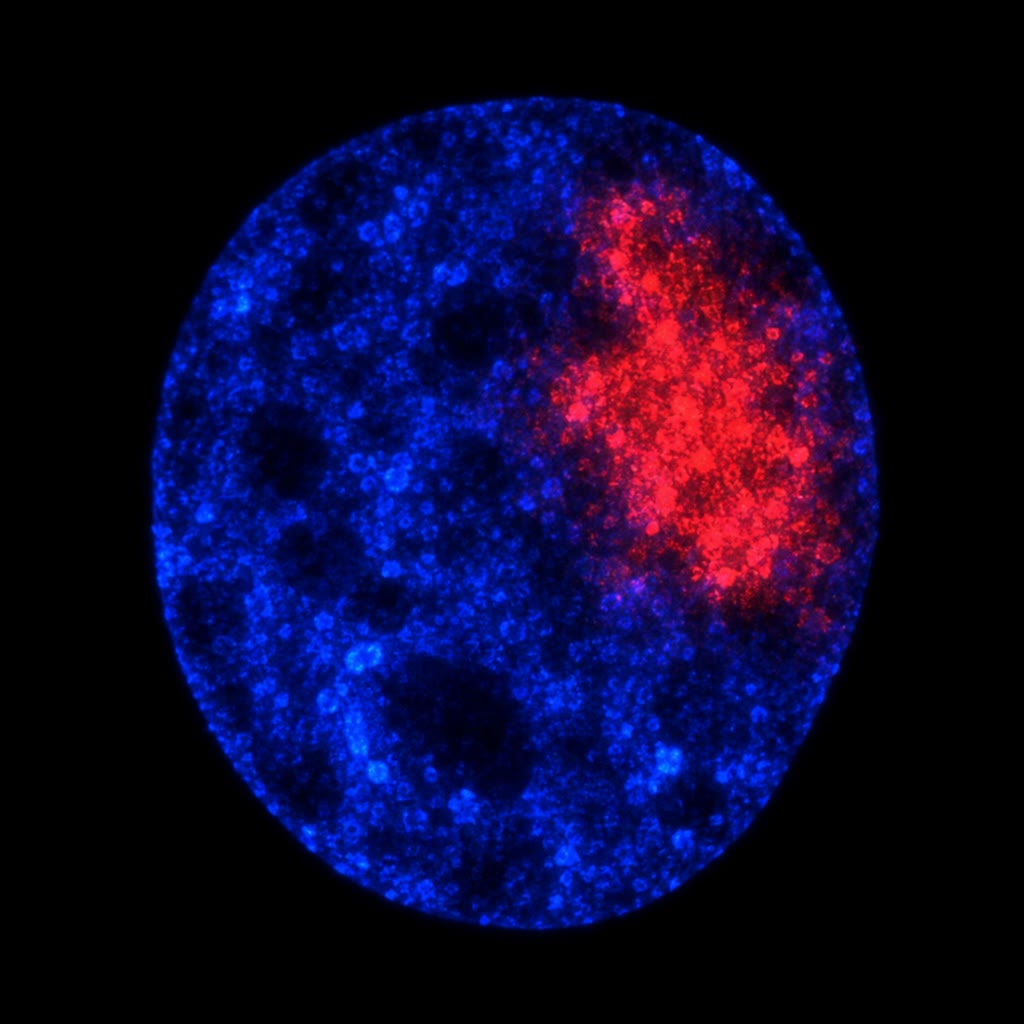
\includegraphics[width=0.36\linewidth]{images/book5/ai/b5-02-lncrna-nucleus.jpg}

{\small Sebuah \omterm{def:b3:rna-regulation:ncrna}{RNA tak penyandi panjang} sedang bekerja: transkrip \emph{\omterm{def:b3:chromatin-epigenetics:x-inactivation}{Xist}}
(merah), yang dideteksi dengan hibridisasi berpendar, menyelimuti wilayah satu
kromosom X di dalam nukleus sel betina (DNA berwarna biru).}
\end{omfigure}

\begin{remark}[Apa yang dibeli kendali pascatranskripsi]\label{rem:b3:rna-regulation:why}
Kendali transkripsi bekerja lewat nukleus, dengan tundaan beberapa menit
sampai beberapa jam sebelum RNA duta baru dibuat, diekspor, dan ditranslasi.
Kendali atas RNA dutanya sendiri bekerja di tempat proteinnya dibutuhkan,
dalam hitungan detik sampai menit, dan dapat bersifat setempat: sebuah
dendrit tunggal mentranslasi satu RNA duta pada satu sinaps, tepi depan
sebuah fibroblas membuat aktin di tempat ia merayap. Kendali itu juga
mengubah satu gen menjadi banyak protein, dan memungkinkan satu isyarat ---
besi, sebuah asam amino, sebuah \omterm{def:b3:rna-regulation:ncrna}{mikroRNA} --- menyelaraskan ratusan RNA duta
sekaligus tanpa menyentuh satu promotor pun.
\end{remark}

\section{Latihan}

\begin{exercise}[$\star$]\label{exo:b3:rna-regulation:1}
Bedakanlah miRNA, \omterm{def:b3:rna-regulation:ncrna}{siRNA}, dan \omterm{def:b3:rna-regulation:ncrna}{piRNA} menurut asal, panjang, ketergantungannya
pada \omterm{def:b3:rna-regulation:rnai}{Dicer}, dan apa yang dilakukannya pada sasarannya.
\end{exercise}

\begin{exercise}[$\star$]\label{exo:b3:rna-regulation:2}
Telusurilah biogenesis sebuah \omterm{def:b3:rna-regulation:ncrna}{mikroRNA} dari gennya sampai ke RNA duta yang
tertekan, sambil menyebutkan enzim pada tiap pemotongan.
\end{exercise}

\begin{exercise}[$\star$]\label{exo:b3:rna-regulation:3}
Mengapa penyuntikan RNA sens \emph{unc-22} ke dalam cacing membungkam gen itu
pada percobaan awal, dan apa yang diubah Fire dan Mello?
\end{exercise}

\begin{exercise}[$\star$]\label{exo:b3:rna-regulation:4}
Apa yang terjadi pada feritin dan pada reseptor transferin ketika sebuah sel
kelaparan besi? Langkah ekspresi yang mana yang dikendalikan pada
masing-masing kasus?
\end{exercise}

\begin{exercise}[$\star\star$]\label{exo:b3:rna-regulation:5}
Sebuah RNA duta berwaktu paruh \qty{2}{h} dan dibuat pada $5$
molekul tiap menit. Hitunglah kadar tunaknya, lalu kadar dan waktu paruhnya
ketika sebuah \omterm{def:b3:rna-regulation:ncrna}{mikroRNA} melipatduakan laju peluruhannya.
\end{exercise}

\begin{exercise}[$\star\star$]\label{exo:b3:rna-regulation:6}
Sebuah benih sepanjang tujuh nukleotida cocok dengan urutan acak dengan
peluang $4^{-7}$. Di dalam himpunan \num{20000} RNA duta yang daerah tak
tertranslasi 3$'$-nya rata-rata \qty{1000}{nt}, berapa tapak yang dicocoki
satu benih \omterm{def:b3:rna-regulation:ncrna}{mikroRNA} secara kebetulan? Kalau begitu, apa yang membedakan
sasaran yang sungguhan?
\end{exercise}

\begin{exercise}[$\star\star$]\label{exo:b3:rna-regulation:7}
Ramalkanlah jenis kelamin seekor lalat (a) yang bermutasi \emph{tra} hilang
fungsi dan berkromosom X dua; (b) yang mengekspresikan TRA dari transgen yang
terus menyala, dengan satu X; (c) yang sama sekali tanpa \emph{dsx}.
\end{exercise}

\begin{exercise}[$\star\star$]\label{exo:b3:rna-regulation:8}
Sebuah RNA duta protoonkogen lazimnya berwaktu paruh \qty{15}{min}
karena sebuah \omterm{def:b3:rna-regulation:stability}{elemen kaya AU}. Sebuah translokasi kromosom membuang elemen itu
dan waktu paruhnya menjadi \qty{3}{h}. Dengan faktor berapa kadar proteinnya
naik, andaikan translasi dan penguraian proteinnya tak berubah? Mengapa hal
ini bersifat onkogenik walaupun proteinnya normal?
\end{exercise}

\begin{exercise}[$\star\star$]\label{exo:b3:rna-regulation:9}
Sebuah galur laboratorium \emph{Drosophila} tidak memiliki elemen P; sebuah
galur liar membawanya. Ramalkanlah kesuburan keturunan
(a) betina laboratorium $\times$ jantan liar, (b) betina liar $\times$
jantan laboratorium, lalu jelaskan ketaksetangkupannya dengan \omterm{def:b3:rna-regulation:ncrna}{piRNA}.
\end{exercise}

\begin{exercise}[$\star\star\star$]\label{exo:b3:rna-regulation:10}
Dengan \cref{thm:b3:rna-regulation:mirna-kinetics}, kemukakanlah bahwa protein
yang dibuat dari sebuah RNA duta lebih sedikit beriak, secara nisbi, ketika
RNA dutanya berada di bawah kendali \omterm{def:b3:rna-regulation:ncrna}{mikroRNA}, pada kadar RNA duta rata-rata
yang sama. (Proteinnya merata-ratakan RNA dutanya sepanjang umurnya sendiri,
dan RNA dutanya memperbarui diri lebih cepat.) Mengapa sebuah sel mungkin
membayar sebuah \omterm{def:b3:rna-regulation:ncrna}{mikroRNA} dan laju transkripsi yang lebih tinggi demi rata-rata
yang sama?
\end{exercise}

\begin{exercise}[$\star\star\star$]\label{exo:b3:rna-regulation:11}
Pada cacing, RNA polimerase bergantung-RNA membuat \omterm{def:b3:rna-regulation:ncrna}{siRNA} sekunder dari
RNA duta sasarannya; pada mamalia tidak ada polimerase semacam itu.
Ramalkanlah, bagi masing-masing, apakah pembungkaman oleh satu suntikan RNA
beruntai ganda bertahan sepanjang banyak pembelahan sel dan apakah
pembungkaman itu menyebar ke jaringan lain, lalu jelaskan akibat medisnya bagi
obat \omterm{def:b3:rna-regulation:ncrna}{siRNA}.
\end{exercise}

\begin{exercise}[$\star\star\star$]\label{exo:b3:rna-regulation:12}
Sebuah lncRNA yang baru teranotasi diekspresikan di dalam jantung. Rancanglah
percobaan yang akan membedakan (a) sebuah RNA yang berfungsi, (b) tindakan
transkripsi yang berfungsi tetapi RNA-nya tak berarti, dan (c) derau, lalu
katakan hasil apa yang diramalkan masing-masing.
\end{exercise}

\section{Soal: Penakar Waktu Seekor Cacing}

\begin{problem}[{Soal akhir pekan --- sakelar \emph{lin-4}/\emph{lin-14}
cacing yang ditakar dengan kinetika RNA dutanya, sebuah RNA suntikan yang
terencerkan sepanjang pembelahan embrio lalu diselamatkan oleh penguatan,
regulon besi yang dikuantifikasi, dan sebuah penghitungan penyambungan,
berakhir pada faktor penekanannya, waktu paruh sakelarnya, dan cacah
pembelahan yang dilalui isyarat yang tak diperkuat}]
\label{pb:b3:rna-regulation:1}
Data: RNA duta \emph{lin-14} dibuat pada $k = 3$ molekul tiap
menit tiap sel dan berwaktu paruh \qty{40}{min}. Protein LIN-14 dibuat pada
$\beta = 2$ tiap RNA duta tiap menit dan berwaktu paruh
\qty{3}{h}. Sejak awal tahap larva kedua, RNA \emph{lin-4}
menumpuk dan menambahkan suku peluruhan $\gamma' R = 3\gamma$ pada RNA
dutanya dan, dengan menghalangi inisiasi, memparuhkan $\beta$. Embrio cacing
berkembang dari satu sel menjadi kira-kira \num{550} sel saat menetas; seekor
dewasa memiliki \num{959} sel somatik.

\medskip
\noindent\textbf{Bagian I --- RNA dutanya.}
\begin{enumerate}
  \item Hitunglah $\gamma$ dan kadar tunak RNA duta \emph{lin-14}
        sebelum \emph{lin-4} muncul.
  \item Hitunglah laju penguraian proteinnya dan kadar tunak protein
        LIN-14.
  \item Begitu \emph{lin-4} hadir, hitunglah kadar RNA duta yang baru
        dan tetapan waktu RNA duta yang baru.
  \item Hitunglah keadaan tunak protein yang baru, dan faktor penekanan
        keseluruhan pada proteinnya.
  \item Berapa lama sesudah \emph{lin-4} muncul RNA dutanya mencapai
        separuh jalan menuju kadar barunya? Dan proteinnya --- langkah mana
        yang membatasi kecepatan sakelarnya?
  \item Percobaan aslinya mendapati proteinnya sudah lenyap sedangkan
        mRNA-nya masih terdeteksi. Apakah hal itu selaras dengan angka
        Anda? Berapa bagian RNA dutanya yang tersisa?
\end{enumerate}

\medskip
\noindent\textbf{Bagian II --- Pengenceran dan penguatan.}
\begin{enumerate}[resume]
  \item Gonad seekor cacing disuntik $10^{6}$ molekul RNA
        beruntai ganda, yang dibagi sama rata di antara \num{250}
        telur. Berapa molekul tiap telur?
  \item Andaikan molekulnya sekadar dibagi-bagi pada tiap pembelahan,
        berapa molekul yang dipegang tiap sel anak cacing bersel \num{550}?
        Sesudah berapa pembelahan lanjutan rata-ratanya jatuh di bawah
        satu tiap sel?
  \item Fire dan Mello melihat pembungkaman pada seluruh tubuh hewan itu
        dan pada keturunannya, pada beberapa molekul tiap sel. Jelaskanlah
        apa yang ditambahkan RNA polimerase bergantung-RNA pada uraian
        tersebut, dan mengapa pengaruhnya toh memudar sesudah beberapa
        generasi.
  \item Di dalam sel mamalia yang tanpa polimerase semacam itu, sebuah
        transfeksi \omterm{def:b3:rna-regulation:ncrna}{siRNA} memasukkan \num{5000} duplek ke dalam sel yang
        membelah tiap hari; \omterm{def:b3:rna-regulation:rnai}{RISC-nya} mantap tetapi terencerkan oleh
        pembelahan. Sesudah berapa hari cacahnya jatuh di bawah \num{100},
        yakni kira-kira cacah yang dibutuhkan bagi pembungkaman yang
        berdaya guna?
  \item Sebuah \omterm{def:b3:rna-regulation:ncrna}{siRNA} terapeutik terhadap RNA duta hati diberikan sekali
        dan bekerja selama enam bulan. Hepatosit jarang membelah.
        Jelaskanlah mengapa mekanisme pertanyaan 10 tidak membatasinya, dan
        apa yang membatasinya.
  \item Sebuah benih sepanjang tujuh nukleotida cocok secara acak sekali
        tiap $4^{7}$ nukleotida. Transkriptom cacing memiliki sekitar
        \qty{20}{Mb} urutan tak tertranslasi 3$'$. Berapa kecocokan benih
        kebetulan yang dimiliki \emph{lin-4}, dan bagaimana para ahli
        genetika tahu sasaran mana yang penting?
\end{enumerate}

\medskip
\noindent\textbf{Bagian III --- Regulon besi.}
\begin{enumerate}[resume]
  \item Di dalam sel kaya besi, RNA duta reseptor transferin berwaktu
        paruh \qty{10}{min}; dengan IRP terikat, \qty{50}{min}.
        Dengan transkripsi yang tak berubah, dengan faktor berapa RNA
        dutanya naik ketika besi menjadi langka?
  \item Kadar RNA duta feritin tak berubah tetapi translasinya
        turun dari $1$ menjadi $0.05$ protein tiap RNA duta tiap menit
        ketika IRP terikat. Dengan faktor berapa sintesis feritinnya turun?
  \item Gabungkanlah keduanya: dengan faktor berapa nisbah kemampuan impor
        terhadap kemampuan simpan berubah antara keadaan kaya besi dan
        keadaan miskin besi?
  \item Protein IRP1 entah menjadi protein pengikat RNA entah menjadi
        akonitase, bergantung pada apakah ia memegang gugus besi--belerang.
        Jelaskanlah mengapa hal itu menjadikannya pengindera besi itu
        sendiri dan bukan pengindera sebuah hormon.
  \item Seorang pasien membawa mutasi IRE feritin yang meniadakan
        pengikatan IRP. Ramalkanlah kadar feritinnya, besi serumnya, dan
        mengapa lensa matanya terkena.
  \item Jelaskanlah dalam satu kalimat mengapa jepit rambut yang sama dapat
        mengaktifkan pada satu kedudukan dan menekan pada kedudukan lain.
  \item IRP2 tidak memiliki gugus besi--belerang; ketika besi tinggi ia
        dimusnahkan oleh ligase ubikuitin yang kemantapannya sendiri
        menuntut besi dan oksigen. Mengapa sebuah sel mungkin memelihara
        dua pengindera yang kimianya begitu berbeda?
\end{enumerate}

\medskip
\noindent\textbf{Bagian IV --- Menghitung isoform.}
\begin{enumerate}[resume]
  \item \emph{Dscam} memiliki blok ekson dengan 12, 48, 33, dan 2 pilihan
        yang saling meniadakan. Berapa isoformnya? Andaikan tiap neuron
        mengekspresikan sekitar $50$ isoform secara acak, berapa peluang
        dua neuron tertentu berbagi sedikitnya satu? (Pakailah $1 - (1 -
        50/N)^{50}$.)
  \item Mengapa sebuah neuron beruntung memiliki isoform yang hampir pasti
        tidak dimiliki tetangganya?
  \item Sebuah gen dengan $n$ ekson kaset, yang masing-masing disertakan
        atau dilewati secara bebas, memberi berapa RNA duta? Berapa untuk
        $n = 10$? Mengapa cacah yang sesungguhnya pada sebuah tipe sel
        biasanya jauh lebih kecil?
  \item Pada lalat, mengapa betina berkromosom X dua tetapi beralel
        \emph{Sxl} nol mati, bukan sekadar berkembang sebagai
        jantan? (Tinjaulah apa lagi yang dikendalikan sistem penghitung X
        itu: \omterm{def:b3:chromatin-epigenetics:x-inactivation}{kompensasi dosis} gen terpaut-X.)
  \item SXL memacu penyambungan produktif transkripnya sendiri.
        Jelaskanlah mengapa hal itu menjadikan keputusan jenis kelamin
        sebuah ingatan yang bertahan sesudah isyarat penghitung X, yang
        hanya hadir pada embrio dini, lenyap, lalu kaitkanlah dengan
        sakelar yang menopang diri pada
        \cref{ch:b3:chromatin-epigenetics}.
  \item Ringkaskanlah penakar waktunya: faktor penekanan protein LIN-14
        (pertanyaan~4), waktu paruh sakelar RNA dutanya
        (pertanyaan~5), dan cacah pembelahan yang dilalui isyarat yang tak
        diperkuat sebelum jatuh di bawah satu molekul tiap sel
        (pertanyaan~8).
\end{enumerate}
\end{problem}
